\chapter{Bipolar Junction Transistor}

\section{Electronic Symbol}

The arrow represents the direction of current.

\begin{figure}[H]
  \centering
  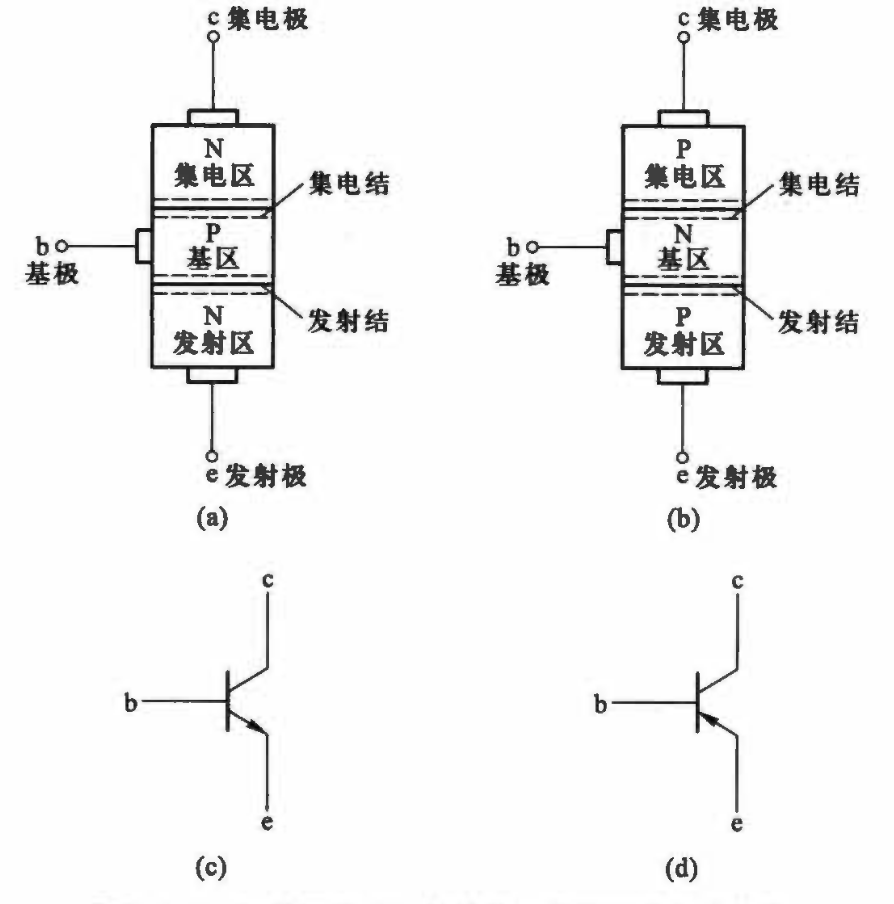
\includegraphics[width=0.7\linewidth]{figures/BJT-Symbol}
\end{figure}

\section{Control Principle}

\begin{figure}[H]
  \centering
  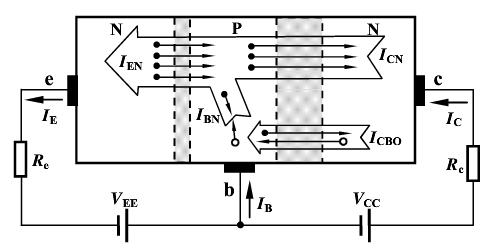
\includegraphics[width=0.7\linewidth]{figures/BJT-control-principle}
\end{figure}

\begin{equation*}
  \begin{aligned}
    \alpha &= \dfrac{I_{c}}{I_e} \quad\quad 
    \beta &= \dfrac{I_{c}}{I_{b}} \quad\quad 
    \alpha &= \dfrac{\beta}{1 + \beta} \quad\quad
    I_e &= \left( 1 + \beta \right) I_b
  \end{aligned}
\end{equation*}

\begin{equation*}
  \begin{aligned}
    I_E = I_{ES} \exp \left( V_{BE} / V_T \right) \quad\quad V_T = 26 \si{mV}
  \end{aligned}
\end{equation*}

\section{Three Types of Amplifier Circuit}

\begin{figure}[H]
  \centering
  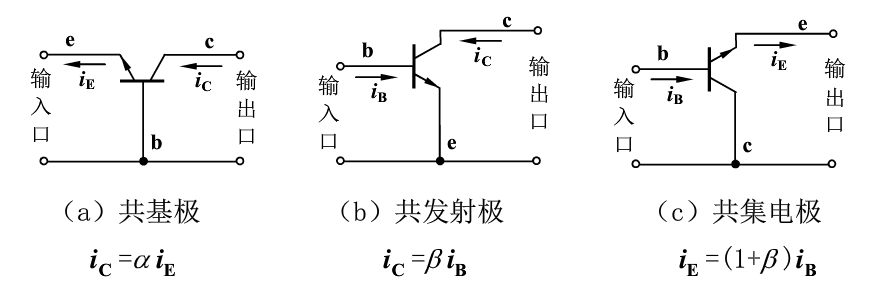
\includegraphics[width=0.9\linewidth]{figures/BJT-three-types}
\end{figure}

\section{Static Working Point}

\begin{figure}[H]
  \centering
  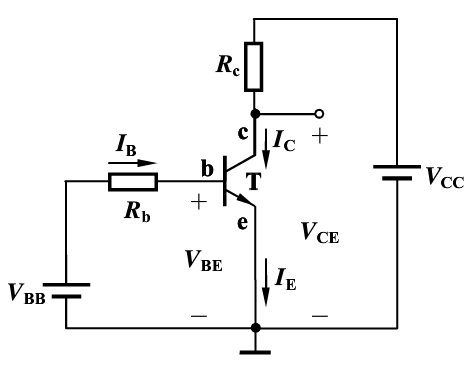
\includegraphics[width=0.4\linewidth]{figures/BJT-static}
\end{figure}

\begin{equation*}
  \begin{aligned}
    & I_{BQ} = \dfrac{V_{BB} - V_{BEQ}}{R_b} \\
    & V_{BEQ} = 0.7 \  \mathrm{V} \\
    & I_{CQ} = \beta I_{BQ} \\
    & V_{CEQ} = V_{CC} - I_{CQ} R_{C}
  \end{aligned}
\end{equation*}

Note that the static working point is not associated with small signals discussed below.

\section{Determine the working state of BJT}

$\beta = 80, V_{BE} = 0.6 \si{V}$

\begin{figure}[H]
  \centering
  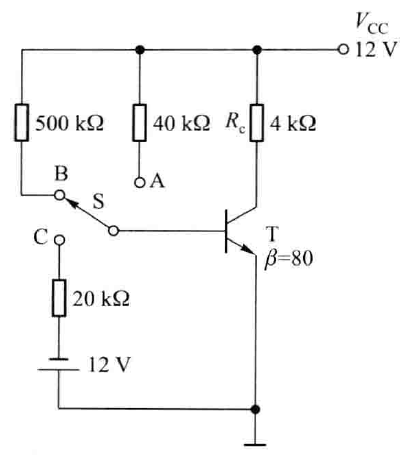
\includegraphics[width=0.5\linewidth]{figures/Working-State-BJT}
\end{figure}

$S \rightarrow A$

\begin{equation*}
  \begin{aligned}
    I_B = \dfrac{\left( 12 - 0.6 \si{V} \right)}{40 \si{k \Omega}} = 0.3 \si{mA} \quad\quad
    I_{CS} = \dfrac{V_{CC}}{R_C} = 0.038 \si{mA} \quad\quad
    I_{BS} = \dfrac{I_{CS}}{\beta} = 3 \si{mA} 
  \end{aligned}
\end{equation*}

Since

\begin{equation*}
  \begin{aligned}
    I_B > I_{BS}
  \end{aligned}
\end{equation*}

BJT works in \textbf{saturation} mode.

$S \rightarrow B$

\begin{equation*}
  \begin{aligned}
    I_B = \dfrac{\left( 12 - 0.6 \si{V} \right)}{500 \si{k \Omega}} = 0.023 \si{mA} \quad\quad
    I_{CS} = \dfrac{V_{CC}}{R_C} = 0.038 \si{mA} \quad\quad
    I_{BS} = \dfrac{I_{CS}}{\beta} = 3 \si{mA} 
  \end{aligned}
\end{equation*}

Since

\begin{equation*}
  \begin{aligned}
    I_B < I_{BS}
  \end{aligned}
\end{equation*}

BJT works in \textbf{active} mode.

$S \rightarrow C$, since

\begin{equation*}
  \begin{aligned}
    V_B < V_E
  \end{aligned}
\end{equation*}

The Emitter-Base Junction is reverse biased, BJT works in \textbf{cutoff} mode.

\section{Model of Small Signal}

\begin{figure}[H]
  \centering
  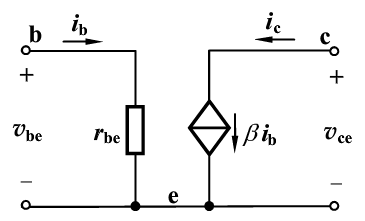
\includegraphics[width=0.5\linewidth]{figures/BJT-small-signal}
\end{figure}

When $T = 300 \  \mathrm{K}$

\begin{equation*}
  \begin{aligned}
    r_{be} = 200 \si{\Omega} + \left( 1 + \beta \right) \dfrac{26 \si{mV}}{I_{EQ} \left( \mathrm{mA} \right)} 
  \end{aligned}
\end{equation*}

\section{Compound Transistor}

\begin{figure}[H]
  \centering
  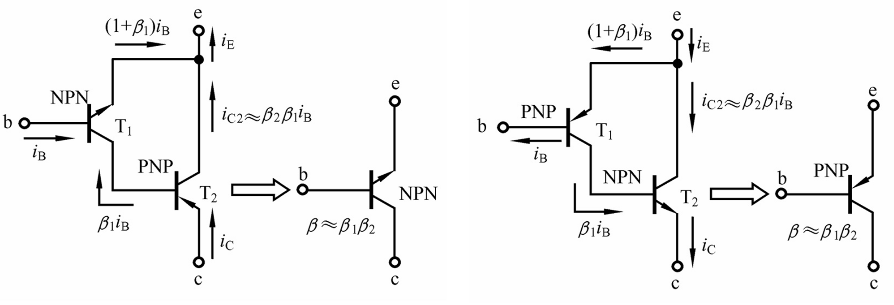
\includegraphics[width=\linewidth]{figures/BJT-compound}
\end{figure}

Noted that the emitter and base of compound transistor is exactly the same as the first transister's.

%%% Local Variables:
%%% mode: latex
%%% TeX-master: "Analogue_Electronics"
%%% End:
